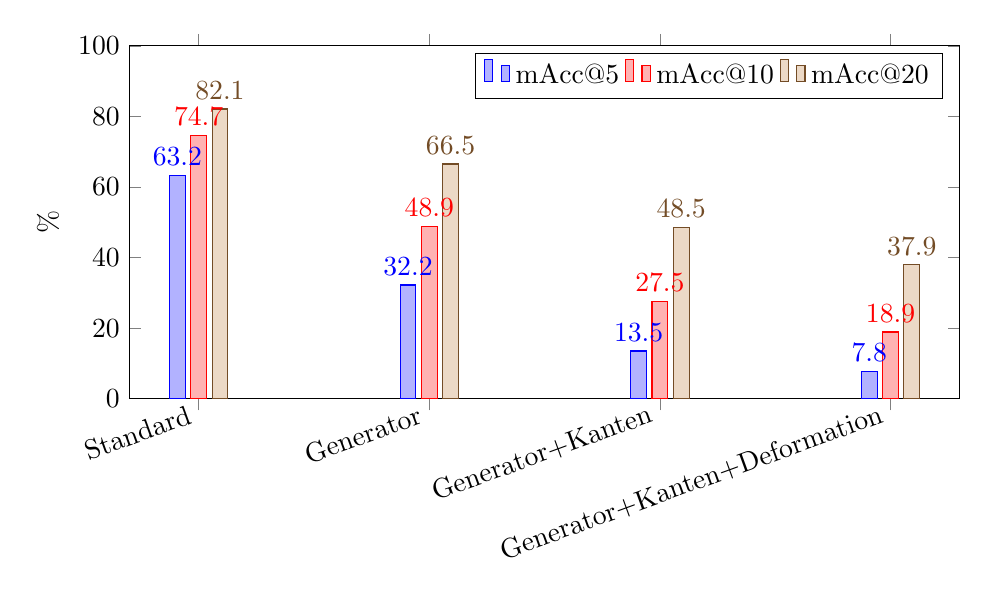
\begin{tikzpicture}
    \begin{axis}[
        ybar,
        bar width=0.2cm,
        width=\textwidth,
        height=0.5\textwidth,
        ylabel={\%},
        symbolic x coords={Standard, Generator, Generator+Kanten, Generator+Kanten+Deformation},
        xtick=data,
        x tick label style={rotate=20, anchor=east}, % <--- hier Labels drehen
        legend style={at={(0.98,0.98)}, anchor=north east, legend columns=-1},
        nodes near coords,
        ymin=0, ymax=100
    ]
        \addplot coordinates {(Standard,63.2) (Generator,32.2) (Generator+Kanten,13.5) (Generator+Kanten+Deformation,7.8)};
        \addplot coordinates {(Standard,74.7) (Generator,48.9) (Generator+Kanten,27.5) (Generator+Kanten+Deformation,18.9)};
        \addplot coordinates {(Standard,82.1) (Generator,66.5) (Generator+Kanten,48.5) (Generator+Kanten+Deformation,37.9)};
        \legend{mAcc@5,mAcc@10,mAcc@20}
    \end{axis}
\end{tikzpicture}
